\begin{center}\large\textbf{Readings: Chapter 7 (for 7.4 read if interested)}\\
\normalsize \end{center}
\large ~\hrulefill
~\\
\normalsize
We saw in the 2-sample t-test we may have interest in testing if two population variances are equal (i.e. $\sigma^2_1=\sigma^2_2$).\\~\\
To investigate this, we first start by looking at inference for a single population variance.\\~\\
\large \textbf{Inference for }$\sigma^2$ \normalsize\\~\\
To make inference for $\sigma^2$ we need a corresponding statistic...\\~\\~\\~\\~\\
This is `unbiased' for $\sigma^2$,\\~\\~\\~\\~\\~\\
To create a CI or HT, we need to know the \underbar{~~~~~~~~~~~~~~~~~~~~~~~~~~~~~~~~~~~~~~~~~~~~~~~~~~~~~~~~~~~~~~~~~~~~~~~~~~~~~~~~~~~~~~~~~~~~~}\\~\\
Theorem:  If $Y_i\sim^{iid}N(\mu,\sigma^2)$ (i.e. a RS from a normal parent population) then\\~\\~\\~\\~\\~\\~\\~\\~\\
Note: Large $n$ will not relax this assumption!  We must have the assumed normality here!
\begin{flushleft}
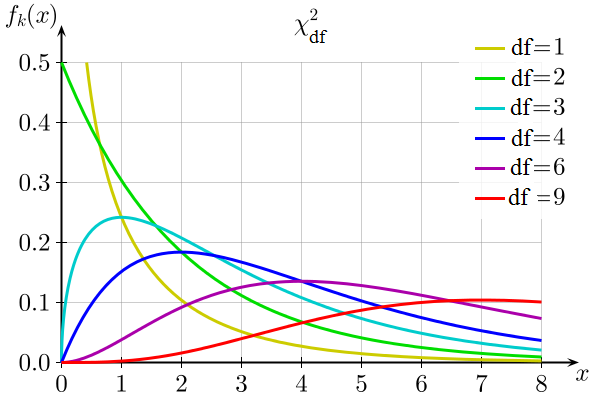
\includegraphics[scale=0.6]{chisquares}
\end{flushleft}~\\
Mean = df, Variance = 2(df)\\~\\
How can we make a $(1-\alpha)100\%$ CI for $\sigma^2$?

\newpage

To get the $\chi^2_L$ or $\chi^2_U$ values in SAS we can do the following:
\begin{small}
\begin{verbatim}
*Syntax     PROBCHI(x,df)        P(Chi^2_df <x) = returned value
The The PROBCHI function returns the probability that an observation from a chi-square distribution, with
degrees of freedom df is less than or equal to x. This function accepts a noninteger degrees of freedom 
parameter df if needed);

*Syntax     QUANTILE(dist, probability, parm-1,...,parm-k)       P(dist<= value returned) = probability 
The QUANTILE function computes the probability from various continuous and discrete distributions
`probability' is a numeric constant, variable, or expression that specifies the value of a random variable.
parm-1,...,parm-k are optional shape, location, or scale parameters appropriate for the specific distribution.;


*Find some probabilities and quantile values from a chi-square;
data chisq;
prob1 = probchi(2,2); *Probability chi-sq 2 is less than its mean --- P(Chi^2_2<2);
prob2 = probchi(12.8,4); *P(Chi^2_4<12.8);

quant1 = quantile('chisq',0.95,11); *0.95 quantile from a chi^2_11;
quant2 = quantile('chisq',0.99,15); *0.99 quantile from a chi^2_15;
run;

proc print data=chisq;
title 'Chi-Square values';
run;
\end{verbatim}
\end{small}

\begin{center}
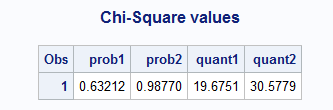
\includegraphics[scale=0.8]{chivalues}
\end{center}

Example:  A dairy processing company claims that the variance of the amount of fat in the whole milk processed by the company is 0.25 $g^2$.  You collect a sample of 41 milk containers and find a sample variance of 0.27 $g^2$.  Find a 90\% CI for $\sigma^2$ = true variance of the amount of fat in the company's whole milk.  What do you think of the company's claim?  Useful values: $P(\chi^2_{40}>55.758)=0.05, P(\chi^2_{40}>26.509)=0.95$ 

\newpage

A hypothesis test for $\sigma^2=\sigma^2_0$ could be done using the test statistic $\chi^2 = \frac{(n-1)s^2}{\sigma^2_0}$.  We won't cover this in class.\\~\\

\textbf{Both the CI and the HT rely heavily on the normality assumption.  If normality does not hold then the interval and test will not be valid!!!  In fact, they perform very poorly (they are not robust to this assumption being violated).}\\~\\


\large \textbf{Inference for two variances}, $\sigma^2_1$ and $\sigma^2_2$ \normalsize\\~\\
Now we are ready to compare two variances (as is needed in the two-sample t-test).  \\~\\
Theorem:  If $Y_i\sim^{iid}N(\mu_1,\sigma^2_1)$ ($i=1,...,n_1$) and $X_i\sim^{iid}N(\mu_2,\sigma^2_2)$ ($i=1,...,n_2$) where the $Y$'s and $X$'s are independent then\\~\\~\\~\\~\\~\\~\\~\\~\\~\\~\\~\\~\\

\begin{flushleft}
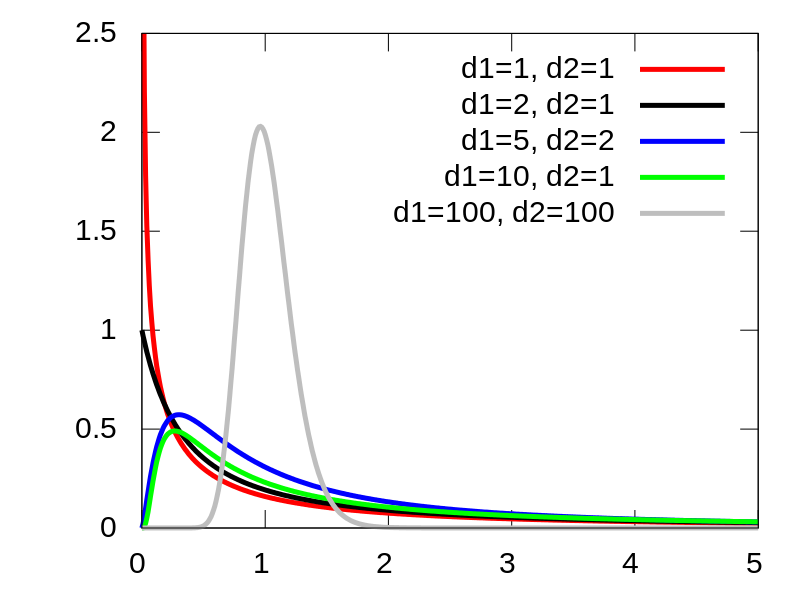
\includegraphics[scale=0.3]{fdist}
\end{flushleft}~\\

\newpage

Notice, when comparing variances we are looking at the ratio $\frac{\sigma^2_1}{\sigma^2_2}$ rather than $\sigma^2_1-\sigma^2_2$.  This is because we know the distribution of the statistic above which involves ratios rather than differences.  What value is of interest for this ratio?\\~\\~\\~\\~\\
How can we make a $(1-\alpha)100\%$ CI for $\sigma^2$?

\newpage



To get the $F_L$ or $F_U$ values in SAS we can do the following:
\begin{small}
\begin{verbatim}
*Syntax    PROBF(x,ndf,ddf)    P(F_df1,df2<x) = returned value
The PROBF function returns the probability that an observation from an F distribution, 
with numerator degrees of freedom ndf (our df1) and denominator degrees of freedom ddf (our df2)
is less than or equal to x. 

*Find some probabilities and quantile values from an F distribution;
data f;
prob1 = probf(10,4,2); *Probability F_4,2 is less than 10 --- P(F_4,2<10);
prob2 = 1-probf(22,3,18); *P(F_3,18>22);

quant1 = quantile('f',0.95,4,2); *0.95 quantile from an F_4,2;
quant2 = quantile('f',0.99,3,18); *0.99 quantile from an F_3,18;
run;

proc print data=f;
title 'F values';
run;
\end{verbatim}
\end{small}

\begin{center}
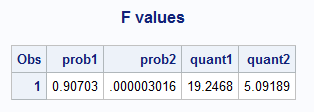
\includegraphics[scale=0.7]{fvalues}
\end{center}

Example:   A company is comparing methods for producing pipes and wants to choose the method with the least variability. It has taken a sample of the lengths of the pipes using both methods and found the following data and summaries.  Find a 99\% CI for the ratio of the variances.  Values: $P(F_{11,14}>4.508)=0.005,P(F_{11,14}>0.196)=0.995,P(F_{14,11}>5.103)=0.005,P(F_{14,11}>0.222)=0.995$
\begin{center}
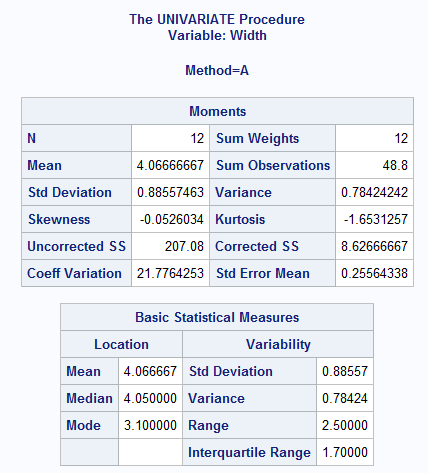
\includegraphics[scale=0.6]{pipes1}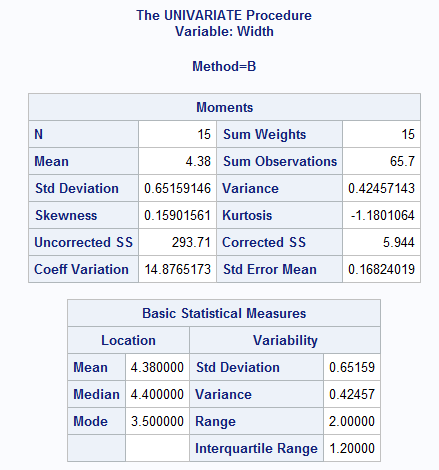
\includegraphics[scale=0.6]{pipes2}
\end{center}

\newpage

The hypothesis test for the ratio of the variances is summarized below:
\begin{center}
\begin{tabular}{c|c|c|c}
Null & Alternative & Test Stat & RR\\\hline
$H_0:\sigma^2_1\leq\sigma^2_2$ & $H_A:\sigma^2_1>\sigma^2_2$ & &\\
$H_0:\sigma^2_1/\sigma^2_2\leq 1$ & $H_A: \sigma^2_1/\sigma^2_2>1$ & $S_1^2/S_2^2$ & $\left\{F_{obs}:F_{obs}\geq F_{\alpha,df1,df2}\right\}$ \\\hline
$H_0:\sigma^2_1=\sigma^2_2$ & $H_A:\sigma^2_1\neq\sigma^2_2$& & \\
$H_0:\sigma^2_1/\sigma^2_2=1$ &  $H_A: \sigma^2_1/\sigma^2_2\neq1$ & $S_1^2/S_2^2$ & $\left\{F_{obs}:F_{obs}\geq F_{\alpha/2,df1,df2}~~or~~F_{obs}\leq F_{1-\alpha/2,df1,df2}\right\}$\\
\end{tabular}
\end{center}

Example: Recall heartrate example from chapter 6.  Conduct an HT for equality of variance at the 0.05 level.  $P(F_{14,10}>3.798)=0.025, P(F_{14,10}>0.316)0.975$
\begin{center}
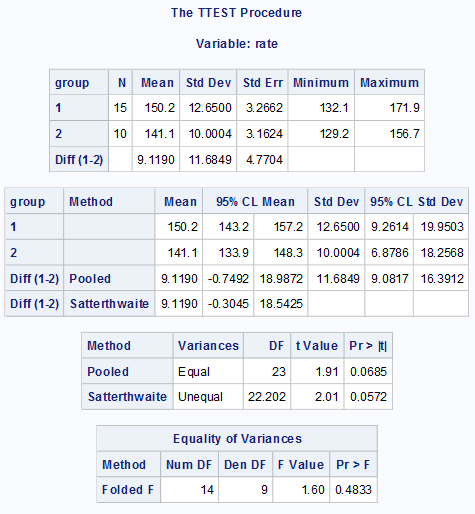
\includegraphics[scale=0.75]{heartratettest}
\end{center}



